\section{Použité technológie a prostredie}
\subsection{OpenCV}
\acrfull{OpenCV} bola pôvodne vydávaná firmou Intel, neskôr výskumným centrom Willow Garage, ktoré vyvíja open source softvér pre aplikácie na poli robotiky. Podporuje frameworky TesorFlow, Torch/PyTorch, Caffe. Knižnica je vydávaná pod BSD licenciou, čo umožňuje jej komerčné používanie. Táto knižnica obsahuje množstvo nástrojov a algoritmov na rozpoznávanie gest, identifikáciu objektov, segmentáciu a rozpoznávanie, spájanie obrazov, sledovanie pohybu, taktiež je vhodná pre implementáciu rozšírenej reality a strojového učenia. OpenCV je podporované v jazykoch C++, Python, Java, C a Matlab. Vývoj je umožnený na operačných systémov Windows, Android, Linux a Mac. \cite{c4}


\subsection{FFmpeg}
Táto knižnica je voľný softvorévý projekt určený na manipulovanie (kódovanie, dekódovanie, multiplexovanie, prehrávanie a streamovanie) s multimediálnymi súbormi. Má voľnú licenciu GNU (General Public License). Výhodou práce s knižnicou FFmpeg je jej rýchlosť a kvalita výstupných dát. Knižnicu využíva aj OpenCV pre spracovanie a distribuovanie obrazovej sekvencie. Obsahuje nástroje na zmenu kvality videa, strihanie, čo napomáha pri kontextovej analýze obrazu.\cite{c9}

\subsection{Python}
Programovací jazyk Python je interpretovaný vysokoúrovňový jazyk, vytvorený v roku 1991. Jeho využitie je široké, od vývoja webových aplikácii, backendu, frontendu cez vedecké a numerické výpočty, tvorbu grafických rozhraní, vývoj softvéru a výučbu a tvorbu biznis aplikácií. V súčasnosti má širokú podporu u programátorov, čo sa odráža aj na prehľadnom zdokumentovaní. Je to open source softvér s množstvom štandardných knižníc, ktoré majú široké využitie v automatizácii, multimédiách, spracovaní obrazu, textu a ďalších sférach IT.\cite{c6}
\subsection{Scikit a Numpy}

\subsubsection{Scikit}
Scikit-learn je knižnica s otvoreným zdrojovým kódom pre strojové učenie pre programovací jazyk Python. Scikit je napísaný v jazyku Python s niektorými algoritmami písanými v Cythone pre zvýšenie výkonu tejto knižnice. Obsahuje rôzne klasifikačné, regresné a zhlukovacie algoritmy, taktiež na modelovanie dát (krížová validácia, výber príznakov, clustering a iné. Je navrhnutá na spoluprácu s numerickou knižnicou NumPy a vedeckou knižnicou SciPy. \cite{c5}

\subsubsection{NumPy}
NumPy je rozšírenie do Pythonu, ktoré nám umožňuje rýchle a efektívne vykonávanie operácií nad poľami homogénnych dát. NumPy pole je multidimenzionálne pole objektov ktoré majú všetky rovnaký typ. V pamäti sa nachádza ako objekt, ktorý smeruje na blok pamäte, ktorý drží informáciu o type údajov v pamäti, počet dimenzií pamäte, veľkosť každej dimenzie a taktiež aj vzdialenosti medzi jednotlivými prvkami pozdĺž každej z osí. Narozdiel od klasického zoznamu, ktorý je implementovaný ako zoznam smerníkov je prehľadávanie NumPy poľa rýchlejšie. klasický zoznam potrebuje na iteráciu poľa prístup cez dva smerníky, čo predĺžuje čas prehľadávania.\cite{c8}


\section{Princípy riešenia}
V prvej časti tejto práce si predstavíme a zároveň porovnáme metódy, ktoré sme zvažovali pri riešení nášho problému. Takisto si zhrnieme aké databázy pohybov máme k dispozícii pre potreby tejto práce, typy databáz, dĺžky jednotlivých videí, vlastnosti a aké druhy aktivít sa v týchto videách nachádzajú. Taktiež je potrebné predstaviť metodológiu spracovania údajov pre zachytenie vhodných vlastností videa na rozpoznanie. Na obrázku \ref{UML1} je znázornená predstava riešenia problému detekcie a rozpoznávania pohybu. Základom je načítanie videí, následne ich predspracovanie na extrakciu príznakov a samotná extrakcia. Konečným krokom v procese by malo byť testovanie a vyhodnotenie aplikácie. 


\begin{figure}[H]
  \centering
  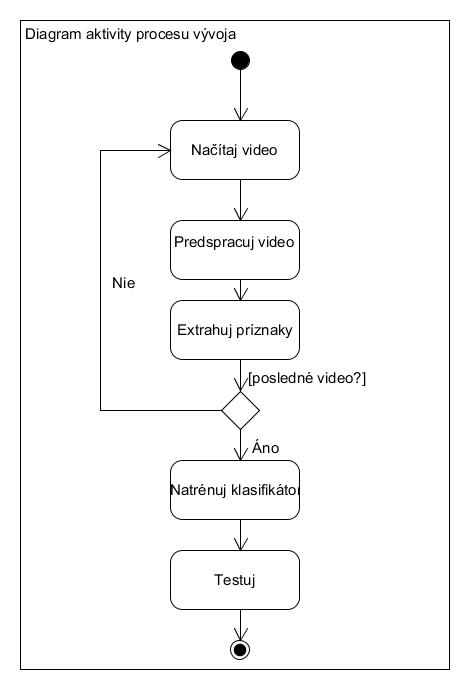
\includegraphics[width=10cm]{img/actTrenovanieKlasifikatora.jpg}
  \caption{Diagram plánu vývoja riešenia}
  \label{UML1}
\end{figure}

\subsection{Spôsob spracovania sekvencie}
Zo zadania vyplýva, že pre získanie príznakov z videa budeme potrebovať videosekvenciu rozdeliť na menšie časti, respektíve ju spracovať do formátu obrázku (.jpg, .png. alebo iné). Jednotlivé snímky z videa sú potrebné na hlbšiu analýzu. Podľa zvoleného datasetu budeme môcť zvoliť či budeme používať celú videosekvenciu, alebo iba jej časť, v ktorej je zrejmý druh pohybu. 

V jednotlivých triedach videí bude potrebné hľadať spoločné a rozdielne znaky na to, aby sme následne vybrali vhodný postup na spracovanie z získanie vhdných príznakov. Knižnica OpenCV neobsahuje metódy ktoré zabezpečia čítanie a prenos obrazu, avšak jej metódy využívajú funkcionalitu ďalšej knižnice FFmpeg, ktorá distribuuje prostredníctvom rozhrania jednotlivé obrazové snímky. 

\subsubsection{Získanie časovo-priestorových vzťahov}
Bude potrebné získať tieto vzťahy na porovnávanie s ďalšími videami, teda určenie vhodného spôsobu na získanie týchto vzťahov. Jedným zo spôsobov je napríklad algoritmus MHI (Motion History Image), ktorý nám môže zabezpečiť tieto príznaky z videa uložiť a ďalej spracovávať. Podľa tohto algoritmu by sme vedeli určiť odkiaľ kam sa aktér z videa pohyboval, akým spôsobom a rýchlosťou, čo môžme považovať za prvé vhodné príznaky pre určenie typu pohybu.\cite{c3} Tento algoritmus si bližšie popíšeme ďalej v tejto práci.

\subsubsection{Extrakcia príznakov}
Extrakcia príznakov je dôležitou časťou pre natrénovanie klasifikátora. Preto je potrebné vybrať príznaky, ktoré nám s čo najvyššou presnosťou zadefinujú konkrétny pohyb, ktorý sa bude vykonávať vo videu. Mali by to byť príznaky, ktoré sú jednoznačné a jedinečné pre každý z druhov pohybu. Preto musíme uvažovať vhodnú metódu extrahovania príznakov, aby sme zaistili diverzitu medzi triedami jednotlivých typov pohybu. K tomu nám bude nápomocná aj kombinácia viacerých spôsobov extrakcie. 

Tieto príznaky budeme extrahovať z predspracovaného zdroja a ukladať na disk pre natrénovanie klasifikátora, prípadne viacnásobné trénovanie a testovanie bude vhodné jednotlivé výsledky ukladať pre neskoršie porovnanie.

\subsubsection{Návrh klasifikátora}
Po úspešnom získaní príznakov z každej videosekvencie bude potrebné natrénovať klasifikátor tak, aby nám každá skupina spracovaných videozáznamov spadala do jednej triedy. Takto natrénovaný klasifikátor budeme potrebovať uložiť pre potreby testovania a porovnávania výsledkov a diverzity jednotlivých skupín. Zároveň budeme potrebovať zvoliť vhodný pomer dát na testovanie a tréning na základe Datábáz, ktoré budeme mať k dispozícii. Z tohto dôvodu budeme potrebovať čo najviac videí, aby bol návrh klasifikačnej metódy čo najpresnejší.


\subsection{Databázy videí}
Na internete je veľké množstvo video databáz s rôznymi pohybmi objektov, ľudí a zvierat.
Výber databázy realizujeme na základe vlastností jednotlivých videí. Videá môžu byť snímané staticky z jedného miesta bez pohybu kamery, staticky s otáčaním kamery, taktiež dynamicky s rôznym pohybom a otáčaním kamery. Výber databázy bude najdôležitejšou súčasťou tejto práce, keďže od nej sa bude odvíjať celý ďalší postup.
\subsubsection{Vlastnosti videa} Dôležitými vlastnosťami videí z databáz sú:
\begin{itemize}
\item \textbf{veľkosť}
\item \textbf{rozlíšenie}
\item \textbf{dĺžka}
\item \textbf{počet videí}
\item \textbf{spôsob snímania}
\item \textbf{formát videa}
\item \textbf{počet objektov}
\end{itemize}

\textbf{Veľkosť} videa ovplyvňuje vo vysokej miere časový úsek určený na spracovanie videa. Z tohto dôvodu je vhodné hľadať databázy videí, ktorých videá majú menšiu veľkosť, čo priamo súvisí s ich rozlíšením, počtom snímkov za sekundu a dĺžkou. Nesmieme ale zabudnúť na to, že video musí byť zreteľné a pohyb detekovateľný.

\textbf{Rozlíšenie} videa je dôležitým faktorom pre spracovnie z hľadiska kvality príznakov a snímkov. Zároveň jeho odporúčaná veľkosť sa líši od konkrétneho spôsobu extrakcie príznakov. Dôležité je, aby obraz konkrétnej aktivity na videu bol jasný a voľným okom rozpoznateľný.

\textbf{Dĺžka} sekvencie sa líši od rozmanitosti jednotlivých pohybov osoby. Niektoré databázy obsahujú videosekvencie s opakovaním pohybov, teda dĺžka videí v týchto databázach je väčšia ako v tam, kde je daná aktivita alebo pohyb zachovaný bez opakovania.

\textbf{Počet videí} môže ovplyvniť výsledok a efektivitu rozpoznávania aktivít. Niektoré databázy obsahujú malé množstvo videí pre jeden konkrétny pohyb (okolo 10 až 20), iné zdroje videosekvencií ich majú aj viac ako 50 pre jeden typ pohybu.

\textbf{Spôsob snímania} v rozpoznávaní pohybu je dôležitou vlastnosťou, keďže nie všetky spôsoby riešenia je možné aplikovať na videá s pohybujúcou sa kamerou a opačne. 

\textbf{Formát videa} súvisí s jeho veľkosťou, avšak formát je možné meniť a konvertovať na nami potrebný rozmer.

\textbf{Počet objektov}, ktoré sa na videu pohybujú a vyhodnocujú vplýva na výkon a rýchlosť rozpoznávania. Tu taktiež nie je možné aplikovať niektoré metódy rozpoznávania.

\subsubsection{Databázy ľudského pohybu}\label{dbludskeho}
Pre potrebu rozpoznávania pohybu osoby existuje viacero databáz, ktoré sme v našej práci uvažovali a testovali:
\begin{itemize}
\item \textbf{HMDB51}
\item \textbf{KTH}
\item \textbf{UCF-Sports}
\item \textbf{Hollywood}
\item \textbf{MSR Action I, II}
\item \textbf{IXMAS}
\item \textbf{WEIZMANN}
\end{itemize}

\textbf{HMDB51} je databáza pohybov v ktorej sa nachádza 51 tried pohybu a gestikulácie ako napríklad česanie vlasov, žuvanie, lezenie, potápanie, chôdza atď. Celkovo obsahuje 6849 videí s rozlíšením 320 x 240 pixelov. Videá sú so statickou aj dynamickou kamerou. Zdrojom videí je YouTube ako aj iné verejne dostupné databázy videí. Videá sú špecifické vysokou diverzitou kvality ako aj pohybu.\cite{c1}

\textbf{KTH} pohybová databáza so šiestimi triedami - chôdza, pomalý beh, beh, boxovanie, kývanie rukou, tlieskanie. V každej z týchto tried sa nachádza 100 čiernobielych videí s rozlíšením 160 x 120 pixelov so statickou kamerou. Videá sú natočené v interiéri ako aj exterieri. \cite{c1}

\textbf{UCF-Sports} obsahuje 9 tried pohybu so 182 videami so statickou aj dynamickou kamerou. Rozlíšenie videí je 720 x 480 pixelov. Videá sú z rôznych športových podujatí vysielaných v televízii - skok do vody, vzpieranie, jazda na koni a iné.\cite{c1} 

\textbf{Hollywood} databáza obsahuje 8 tried - vystúpenie z vozidla, bozkávanie, postavenie sa, sadnutie si a iné. Nachádza sa tam 430 videí s rozlíšením 300 - 400 x 200 - 300 pixelov s dynamickou kamerou a dynamickým pozadím.\cite{c1}

\textbf{MSR Action I, II} obsahujú 3 triedy pohybu so statickou kamerou a 16-timi videami s  rozlíšením 320 x 240 pixelov. Namodelované videá sú určené na detekciu pohybu, nie jeho rozpoznávanie. Vo videách sa nachádza viac ako jeden pohyb. V pozadí sa objavujú aj iné osoby, prípadne objekty ako auto. \cite{c1}

\textbf{IXMAS} alebo \textit{INRIA Xmas Motion Acquisition Sequences} obsahuje 13 tried s rozlíšením 390 x 291. Pohyb je zaznamenávaný z viacerých statických kamier. \cite{c1}

\textbf{WEIZMANN} obsahuje 10 tried pohybu, celkový počet videí je 90. Obsahujú triedy pohybu ako chôdza, beh, kývanie jednou alebo dvomi rukami, skok na mieste a iné. Videá sú natočené so statickou kamerou a pozadím  v interiéri  s rozlíšením 180 x 144. \cite{c1}

\subsection{Možnosti spracovania obrazu}
Na získanie príznakov a potrebu klasifikácie pohybu analyzujeme a zvažujeme konkrétne spôsoby spracovania obrazu z videa. Pre tento účel berieme v úvahu algoritmus \acrfull{mhi} na extrakciu prvotných príznakov a následné spracovanie pomocou \acrfull{hog}. 

Pre zosilnenie našich príznakov a zaručenie vyššej úspešnosti klasifikácie uvažujeme použitie \acrfull{pca}, ktoré taktiež urýchli trénovanie klasifikátora. Takto získané príznaky by sme následne vedeli natrénovať pomocou \acrfull{svm}. Z natrénovanej SVM vieme otestovať úspešnosť klasifikátora, ktorý sme získali a tým sa dostať ku výsledkom a porovnávaniam. 

\subsubsection{Motion History Image} \label{MHIlabel}
\acrshort{mhi} je metódou, ktorá je založená na časovej šablóne. Je to jednoduchá metóda avšak robustná, vhodná na reprezentovanie a analýzu pohybu.\cite{c3}  Táto metóda bola prvýkrát popísaná v dokumente ``An appearance-based representation of action'' od Aarona Bobicka a Jamesa W. Davisa.\cite{c2} Rozpoznávanie akcie pomocou MHI patrí do skupiny prispôsobovania šablóny. V MHI sa informácia pohybu v čase spája do jedného obrázku, kde intenzita pixelov je funkciou histórie pohybu na danej pozícii pixelu. MHI sa vypočítava pomocou aktualizačnej funkcie.\ref{MHIeq}


\begin{figure}[H]
  \centering
  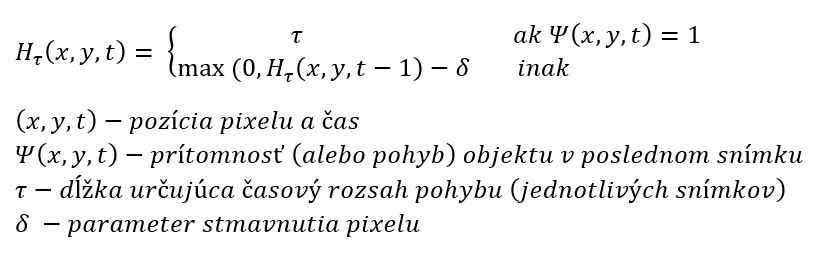
\includegraphics[width=14cm]{img/MHIeq.jpg}
  \caption{Funkcia zmeny pixelov v MHI}
  \label{MHIeq}
\end{figure}

Táto aktualizačná funkcia je volaná pre každý ďalší snímok, ktorý analyzujeme z videosekvencie. Výsledkom tohto výpočtu je skalárny snímok, v ktorom svetlejšie časti obrázku označujú najnovšie menené pixely a tmavšie sú tie, ktoré boli menené dávnejšie z pohľadu pohybu na videu.

To nám umožňuje zaznamenať pohyb z videa do jediného obrázku, v ktorom je vystihnutý celý priebeh videa alebo jeho časti. Táto technika je vhodná na použitie pri videách so statickou kamerou a pozadím.\cite{c10}

\begin{figure}[H]
  \centering
  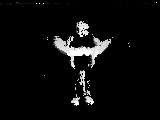
\includegraphics[width=13cm]{img/MHIclap.jpg}
  \caption{Motion History image tlieskania}
  \label{MHIclap}
\end{figure}

Na obrázku \ref{MHIclap} je príklad spracovaného pohybu z videa do MHI, na ktorom môžme vidieť pohyb tela pri akcii tlieskania.

	 

\subsubsection{Histogram of Oriented Gradients} \label{HOGlabel}
HOG je metóda extrakcie príznakov z obrazu. Extrahuje príznaky z každej časti vstupného obrazu. Snaží sa zachytiť tvar štruktúry v regiónoch pomocou prechodov farieb jednotlivých pixelov. Rozdeľuje obraz na menšie spojené časti (napríklad 8 x 8 pixelov)a tie časti do ešte menších blokov z ktorých sa následne zostavuje histogram. Deskriptor je spojenie týchto histogramov. 

Každá z týchto častí  má rovnaký počet orientácií gradientu.  Pre zvýšenie presnosti môžu byť lokálne histogramy normalizované na základe kontrastu a výpočtom miery intenzít naprieč väčšími časťami obrazu, teda bloku. Táto normalizácia vedie k zvýšenej invariantnosti pri zmene osvetlenia alebo tienenia. 

HOG Deskriptor má výhody v tom, že pôsobí na lokálne bunky, je invariantný voči geometrickým a fotometrickým transformáciám. N. Dalal a B. Triggs zistili, že hrubé priestorové vzorkovanie, jemné vzorkovanie a silná lokálna fotometrická normalizácia umožňujú HOG deskriptoru vhodne detekovať ľudské bytosti v obrazoch. 

\paragraph{Výpočet gradientu}

Základným krokom pri HOG algoritme je výpočet gradientových hodnôt. Najbežnejšou metódou je aplikácia 1-D centrovanej diskrétnej masky v horizontálnom alebo aj vertikálnom smere. Táto metóda vyžaduje filtrovanie farieb alebo intenzitu obraz s filtračnými jadrami.

\paragraph{Histogram orientovaných gradientov}
Ďalším krokom je vytvorenie histogramu orientovaných gradientov. Každý pixel v bunke pridáva svoju ováhovanú orientáciu pre orientovaný histogramový kanál, ktorý je vytvorený na základe výpočtu gradientov. Bunky môžu byť obdĺžníkového alebo radiálneho tvaru a histogramové kanály sú rozložené rovnomerne od 0 do 180 alebo 0 - 360 stupňov, záleží od toho, či gradienty môžu nadobúdať aj zápornú hodnotu, alebo nie. 

Podľa výskumov  N. Dalala a B. Triggsa bolo zistené, že najvhodnejší počet kanálov na detekovanie osoby je 9 pri rozsahu 0 - 360 stupňov.

\paragraph{Bloky deskriptorov}
Na zohľadnenie zmien v osvetlení a kontraste musí byť intenzita gradientu lokálne normalizovaná, čo vyžaduje spoločné zoskupovanie buniek do väčších priestorovo prepojených blokov. HOG Deskriptor je následne spojený vektor komponentov normalizovaných histogramov buniek zo všetkých oblastí blokov. Tieto bloky sa prekrývajú, z čoho vyplýva, že každý jedna bunka prispieva voac ako raz do vytvorenia konečného deskriptora. Existujú dva hlavné tvary blokov:

\begin{itemize}
\item \textbf{R-HOG} (Rectangular HOG)
\item \textbf{C-HOG} (Circular HOG)
\end{itemize}


\textbf{R-HOG} - sú štvorcové mriežky reprezentované tromi parametrami:
\begin{itemize}
\item počet buniek v bloku
\item počet pixelov v bunke
\item počet kanálov na histogram bunky
\end{itemize}

V práci N. Dalala a B. Triggsa je uvedené, že optimálne parametre sú štyri pixelové bunky s veľkosťou  8 x 8 na jeden blok (16 x 16 pixelov na blok)s deviatimi histogramovými kanálmi. Bolo taktiež zistené, že menšie vylepšenie vo výkonnosti môže byť nadobudnuté použitím Gaussovho priestorového okna v každom bloku pred zaznamenaním váhovaných histogramov. Lepšiemu výsledku by napomohlo to, že okrajové pixely by boli ováhované nižšími hodnotami. 

\textbf{C-HOG} - sú kruhové bloky, ktoré je možné použiť v dvoch variantoch. Jednou variantou je využitie jednej centrálnej bunky, pri druhej variante je táto bunka uhlovo rozdelená do rovnakých častí. Tieto bloky sú popísané štyrmi parametrami:

\begin{itemize}
\item počet uhlových buniek
\item počet radiálnych buniek
\item polomer stredovej bunky
\item faktor expanzie pre polomer dodatočných radiálnych buniek
\end{itemize}

Podľa zistení N. Dalala a B. Triggsa najvhodnejšie zvoleným spôsobom je vytvorenie dvoch radiálnych buniek so štyrmi uhlovými bunkami, polomerom stredovej bunky 4 pixely a faktor expanzie s hodotou 2. 


\begin{figure}[H]
  \centering
  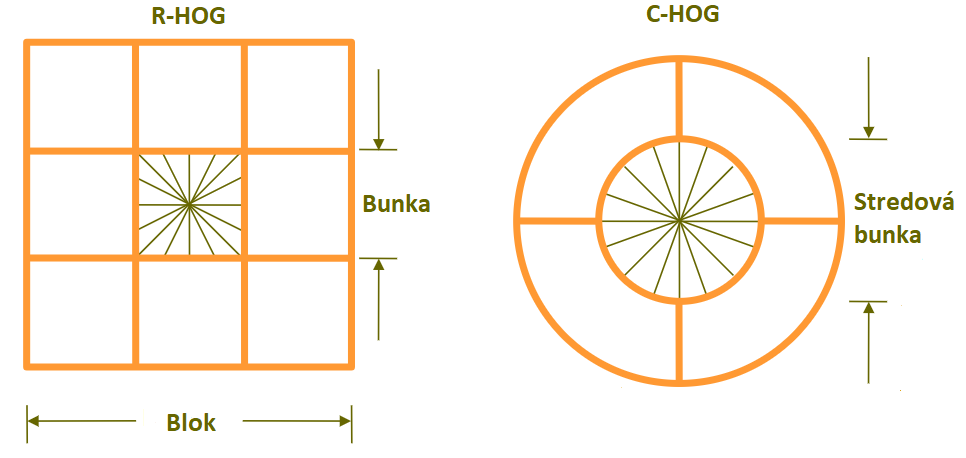
\includegraphics[width=14cm]{img/HOGimg.png}
  \caption{R-HOG a C-HOG}
  \label{HOGimg}
\end{figure}

Na obrázku \ref{HOGimg} môžme vidieť ako vyzerá rozdelenie obrazu podľa R-HOG a C-HOG.

\paragraph{Normalizácia blokov}
Sú štyri rôzne spôsoby normalizácie blokov, ktoré sú popísané na obrázku \ref{HOGnorm}.

\begin{figure}[H]
  \centering
  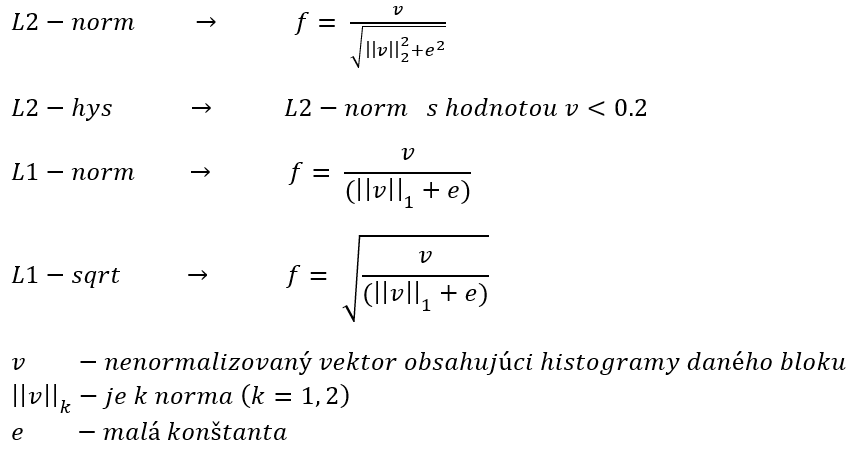
\includegraphics[width=14cm]{img/HOGnorm.png}
  \caption{Metódy normalizácie}
  \label{HOGnorm}
\end{figure}

Schéma \textbf{\textit{L2-hys}} môže byť vypočítaná z \textbf{\textit{L2-norm}}, kde sa výsledok renormalizuje pre vektor \textit{v < 0.2}. Všetky štyri normy majú výrazne lepšie výsledky ako nenormalizované dáta. Tieto údaje sú následne použiteľné ako vektor príznakov pre SVM. \cite{c11}


\subsubsection{Principal Component Analysis} \label{PCAlabel}
Analýza hlavných komponentov (angl. Principal Components Analysis) je metóda štatistiky, ktorá využíva ortogonálnu transformáciu za účelom zmeny prvkov, v ktorých sa vyskytuje korelácia na prvky, kde  sa takáto lineárna korelácia nebude existovať. \acrshort{pca} teda spracováva a upravuje jednotlivé komponenty tak, aby sa ich dimenzia zmenšila, alebo bola nanajvýš rovnaká a zároveň sa snaží zachovať čo najväčšie množstvo informácií o pôvodných premenných. Tento prístup pomáha analyzovať dané dáta v podpriestore, čo nám umožňuje ďalšie spracovanie.

Dôležitou súčasťou v PCA sú vlastné vektory. Sú to nenulové vektory, ktorých smer sa po transformácii pomocou lineárneho operátora nemení, pojem vlastný vektor v PCA obmieňame za hlavný komponent. 

V Computer Vision má táto metóda veľmi dobrý vplyv na dáta charakterizujúce rôzne špecifické tvary, objekty, keďže nám umožňuje zosilniť význam príznakov, ktoré sú pre daný problém dôležité, a tie, ktoré nie sú potrebné, dokáže eliminovať. Táto transformácia teda zvyšuje varianciu hlavných komponentov naprieč všetkými lineárnymi kombináciami vektora, čo napomáha zvyšovať úspešnosť klasifikátora pri riešení rozpoznávania na extrakciu príznakov. Túto metódu navrhol v roku 1901 matematik anglického pôvodu Karl Pearson. Jej rôzne obmenené a vylepšené verzie sa využívajú dodnes v štatistike, \textit{Computer Vision}, robotike a ďalších smeroch.

Pomocou Jordanovej dekompozičnej vety o symetrických maticiach môžme symetrické štvorcové matice zapísať v nasledovnom tvare, ktorý je na obrázku \ref{PCAJord} \cite{c15} \cite{c16}.
\begin{figure}[H]
  \centering
  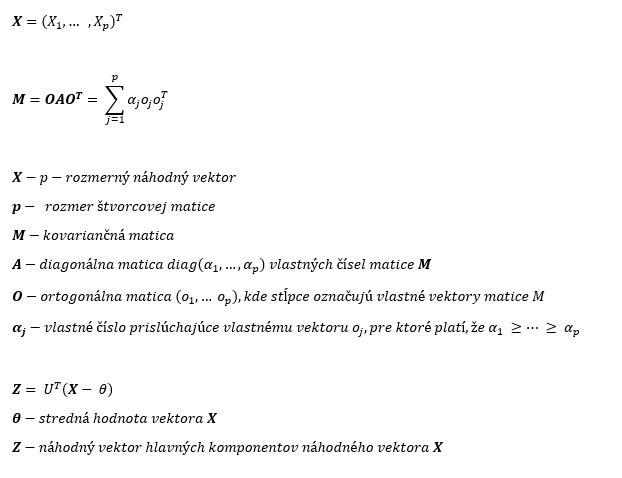
\includegraphics[width=16cm]{img/PCAjordan.png}
  \caption{Definícia Jordanovej matice}
  \label{PCAJord}
\end{figure}

Z tejto matice následne vieme vypočítať vektor hlavných komponentov, viď obrázok \ref{PCAhlav}.

\begin{figure}[H]
  \centering
  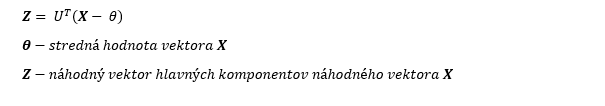
\includegraphics[width=16cm]{img/PCAhlavnekomponenty.png}
  \caption{Výpočet hlavných komponentov}
  \label{PCAhlav}
\end{figure}
\cite{c17}

Redukciou dimenzie vieme dosiahnúť aj kratšiu dobu trénovania klasifikátora ako aj jeho vyššiu úspešnosť. 


\subsubsection{Support Vector Machine} \label{SVMlabel}
SVM je metóda strojového učenia s učiteľom, je vhodná na používanie pri klasifikácii alebo regresnej analýze. Táto metóda na základe trénovacích vzoriek, ktoré sú priradené do jednej z dvoch tried vytvorí model. Tento model je následne schopný priraďovať nové vzorky do jednej z týchto tried, čo z neho robí nepravdepodobnostný binárne lineárny klasifikátor. SVM model reprezentuje vzorky ako body v priestore, tak, že mapuje jednotlivé vstupy do kategórií, ktoré sú v tomto priestore jasne oddelené. Klasifikátor priraďuje nové vzorky podľa toho, ku ktorej z tried majú bližšie v rámci tohto priestoru.

Okrem lineárnej klasifikácie je SVM schopné efektívne riešiť aj nelineárne separovateľné problémy pomocou takzvaného kernel triku. Pokiaľ dáta nie sú pri trénovaní označené, do ktorej kategórie patria, učenie s učiteľom nie je možné, avšak je možné učenie bez učiteľa tak, že algoritmus sa snaží nájsť prirodzené zoskupenie dát a tak ich rozdeliť do kategórií.

SVM algoritmus vytvorili Hava Siegelmann a Vladimir Vapnik. Tento algoritmus má široké využitie a je používaný v priemyselných aplikáciách, počítačovom videní, umelej inteligencii.  \cite{c7}

\paragraph{Definícia algoritmu}
SVM vytvára hyperrovinu \footnote{Podpriestor, ktorý má o jednu dimenziu menej ako priestor, v ktorom sa nachádza.}, alebo viacero hyperrovín, vo vysokorozmernom priestore, ktorý môže byť použitý na klasifikáciu, regresiu alebo iné úlohy. Dobrá separácia sa dosiahne vtedy, keď hyperrovina má veľkú vzdialenosť od najbližšieho trénovacieho bodu akejkoľvek triedy. Teda platí, čím je väčšia vzdialenosť hyperroviny od trénovacích údajov, tým je nižšia chyba klasifikátora pri určovaní triedy testovacej vzorky.\cite{c12}

Keďže nie všetky problémy je možné lineárne separovať, bolo navrhnuté, aby sa priestor, ktorý SVM spracováva rozvrhol do viacrozmerného priestoru, čo uľahčí rozdelenie jednotlivých dát do tried. Pre zanechanie výpočtovej rýchlosti je mapovanie v SVM navrhnuté v pôvodnom priestore, kde sa následne zvolí vhodná kernelová funkcia $ k(x,y)$ . 
Hyperroviny vo viacrozmernom priestore sú definované ako súbory bodov, kde ich vektory majú konštantnú dĺžku. Následne body z proestoru príznakov sú mapované do hyperroviny. 

\paragraph{Lineárny klasifikátor}
Najjednoduchšou možnosťou použitia SVM je prípad lineárneho klasifikátora pre dáta, ktoré je možné lineárne rozdeliť do dvoch tried pomocou hyperroviny. Príklad takéhoto problému je na obrázku \ref{LinSep}.

\begin{figure}[H]
  \centering
  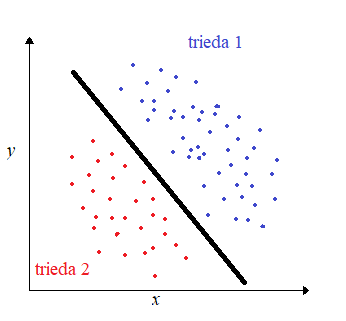
\includegraphics[width=10cm]{img/linsep.png}
  \caption{Príklad lineárne separovateľného problému}
  \label{LinSep}
\end{figure}


\paragraph{Nelineárny klasifikátor}
Na obrázku č. \ref{SVMobr} môžme vidieť lineárne neseparovateľný problém dvoch množín, ktorý sa po pridaní tretej dimenzie stáva lineárne separovateľný. Takýmto spôsobom dokážeme s SVM zatriediť jednotlivé videá z množín do správnych tried. Transformácia do vyššierozmerného priestoru sa nazýva jadrový trik \textit{(angl. kernel trick)}. Pomocou tohto triku vieme lineárne separovať aj lineárne neseparovateľné problémy.\cite{c12}

\begin{figure}[H]
  \centering
  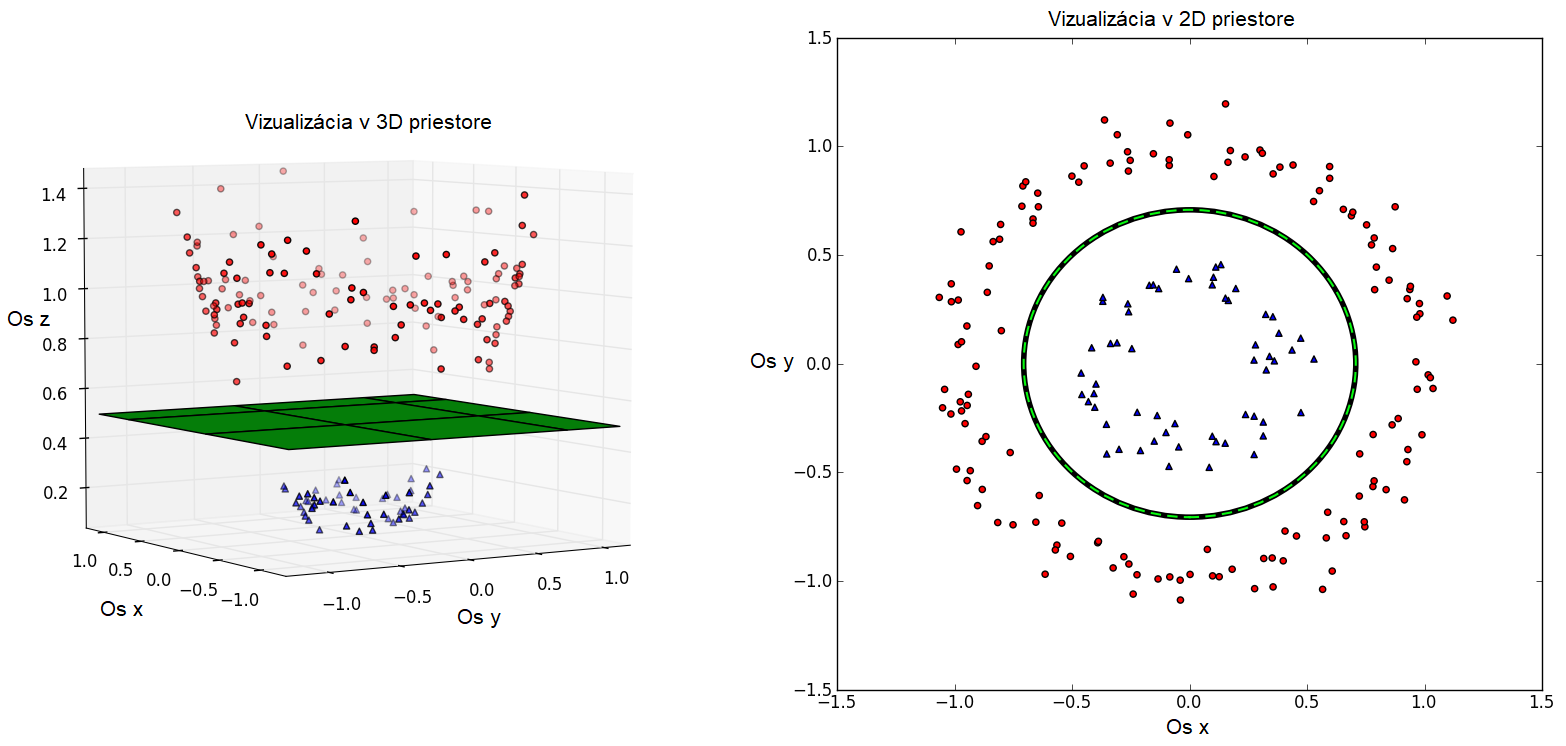
\includegraphics[width=16cm]{img/SVM.png}
  \caption{Rozšírenie dimenzie v SVM}
  \label{SVMobr}
\end{figure}

Medzi najčastejšie používané jadrové funkcie patria:

\begin{itemize}
\item \textbf{Polynóm stupňa \textit{p}}
\item $  K(x,y) = (x.y + 1)^p $
\item \textbf{Radiálne bázové funkcie}
\item $   K(x,y) = e^{(-\|x-y\|^2/2\sigma^2)}  $
\item \textbf{Dvojvrstvová neurónová sieť }
\item $   K(x,y) = \tanh(\kappa x.y - \delta)  $
\end{itemize}



\newpage

\section{Návrh riešenia}
Po oboznámení s teoretickými piliermi tejto práce prejdeme ku konkrétnemu riešeniu témy a implementácii, ktorú sa nám podarilo vytvoriť. Postupne prejdeme jednotlivé kroky vytvárania programu od analýzy datasetov, načítavania a ukladania videosekvencií do obrazkových formátov. Ďalej si ukážeme metódy a spôsoby, ktorými sme následne vzniknuté dáta spracovali pre potrebu výberu príznakov a zatriedenia do jednotlivých tried. Fungovanie programu priblížime aj časťami kódu s popisom, na čo slúži a ako pracuje. Súčasťou tejto kapitoly bude aj krátky popis zmien, ktoré sme počas návrhu tejto implementácie vykonali a samozrejme aj ich dopad na finálne riešenie.

\subsection{KTH Databáza}
Pre naše riešenie sme vyberali z viacerých datasetov, ktoré boli popísané v kapitole \ref{dbludskeho}. Nakoniec sme sa rozhodli pre databázu KTH, v ktorej máme 6 tried pohybu a nachádza sa pri každom z nich 100 videí. Naše rozhodnutie sme učinili takto z viacerých dôvodov. Potrebovali sme dataset, v ktorom sa nachádza veľké množstvo videí, zároveň vo videách sme potrebovali statickú kameru so statickým pozadím, aby sme predišli zvýšenému šumu. V tejto databáze sú pohyby:

\begin{itemize}
\item Boxovanie
\item Mávanie rukami
\item Tlieskanie rukami
\item Beh
\item Pomalý beh
\item Chôdza
\end{itemize}

Pri analýze snímkov sme zistili, že dĺžka videí je od \textit{\textbf{8 do 59 sekúnd}}. Čo pre dané typy pohybov je postačujúci čas na to, aby sme z nich dokázali extrahovať dôležité informácie, ktoré sa tohto pohybu týkajú.  Počet snímkov za sekundu v každom z videí je 25, z tohto dôvodu sme usúdili, že aj v prípade krátkeho videa s dĺžkou 8 sekúnd budeme mať k dispozícii minimálne \textit{\textbf{200}} snímkov. Ďalším dôležitým faktom je, že sa budeme musieť popasovať s podobnosťou pohybov behu, pomalého behu a chôdze, keďže sú veľmi podobné, a ich rozdiel je iba v rýchlosti vykonávania. Je nutné dodať, že v každom z videí sa jednotlivé typy pohybov opakovali viacnásobne, z čoho sme už vopred usudzovali, že na spracovanie nám bude stačiť iba časť videa, čo nám ušetrí čas spracovania dát počas behu programu. 

\begin{figure}[H]
  \centering
  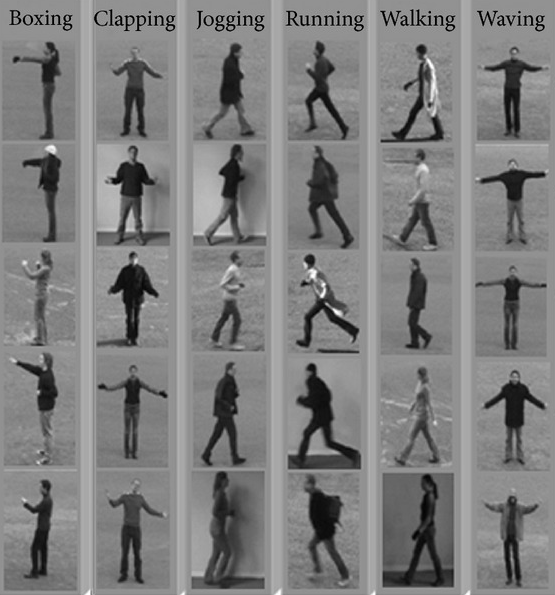
\includegraphics[width=10cm]{img/KTHdataset.png}
  \caption{Jednotlivé pohyby v datasete KTH \cite{c14}}
  \label{KTHobr}
\end{figure}

Na obrázku \ref{KTHobr} vidíme všetky kategórie pohybov, jednotlivé pohyby vykonáva viacero osôb rôznymi spôsobmi, teda je medzi týmito pohybmi aj diverzita, ktorá je určite vhodná na trénovanie pohybu. 

\subsection{Predspracovanie videa}
Na predspracovanie videa a vytiahnutie prvotných príznakov sme sa rozhodli z našich videí vytvoriť obrázky, na ktorých sa bude nachádzať história pohybu. Algoritmus MHI, ktorý sme pri tom použili sme popísali v časti \ref{MHIlabel}. Tento algoritmus sme zvolili na základe toho, že máme databázu videí bez pohyblivého pozadia, teda predídeme šumom na pozadí a budeme sa môcť venovať iba pixelom, ktoré menia svoju pozíciu v rámci videa. Presne to je postačujúca podmienka na to, aby sme bez väčších problémov mohli implementovať funkcionalitu algoritmu MHI na nami zvolený dátový rozsah. Vytvoriť MHI sme sa rozhodli zo všetkých videí, aby sme následne videli, akým spôsobom prebehlo spracovanie, či je možné z MHI vyčítať pohyb a jeho základné znaky. 

\begin{lstlisting}[
  caption={Algoritmus MHI},
  label={MHIcreate},
  language=python
]
def getImage(cam, video_src, vidDir):
  while True:    
    ret, frame = cam.read()
    h, w = frame.shape[:2]
    prev_frame = frame.copy()
    motion_history = np.zeros((h, w), np.float32)
    timestamp = 0
    while True:
      frame_num = frame_num + 1
      ret, frame = cam.read()
      if not ret:
        break
      frame_diff = cv2.absdiff(frame, prev_frame)
      gray_diff = cv2.cvtColor(frame_diff, cv2.COLOR_BGR2GRAY)
      ret, fgmask = cv2.threshold(gray_diff, DEFAULT_THRESHOLD, 1, cv2.THRESH_BINARY)
      timestamp += 1
      # update motion history
      cv2.motempl.updateMotionHistory(fgmask, motion_history, timestamp, MHI_DURATION)
      # normalize motion history
      mh = np.uint8(np.clip((motion_history-(timestamp-MHI_DURATION)) / MHI_DURATION, 0, 1)*255)
      cv2.imshow('motempl', mh)
      print frame_num
      if frame_num == 160:
          frame_num = 0
          imagename = video_src[0:-4] + '.jpg'
          cv2.imwrite(MHI_dir + '\\' + vidDir + '\\' + imagename, mh)
          return
\end{lstlisting}


V tejto ukážke \ref{MHIcreate} kódu je celý proces čítania videa a jeho jednotlivých snímkov za sebou so spracovaním na MHI. Funkcia \textit{getImage} obsahuje tri vstupné parametre:
\begin{itemize}
\item \textbf{cam}
\item \textbf{video\_src}
\item \textbf{vidDir}
\end{itemize}

 \textbf{\textit{cam}}, čo je objekt typu \textbf{\textit{VideoCapture}}, ktorý sa ďalej spracováva po jednotlivých snímkoch. 
 Parameter \textbf{\textit{video\_src}} je názov videosúboru, ktorý sme použili na uloženie obrázku z videa.
 \textbf{\textit{vidDir}} je názov priečinku, v ktorom sa obrázok MHI bude ukladať. 
 Na čítanie snímkov sme použili knižnicu OpenCV, ako aj na spracovanie jednotlivých snímkov do MHI. Dôležitými parametrami, ktoré sme nastavovali boli \textit{frame\_num}, ktorý nám označoval počet prehratých snímkov, pri ktorom sme uložili vyhotovené MHI, ďalej to bol \textit{DEFAULT\_TRESHOLD}, ktorý nám filtroval nepotrebné pixely s veľmi nízkou hodnotou, pri trénovaní a testovaní sme zistili, že hodnota \textit{\textbf{50}} bude dobrá. Akonáhle bol tento parameter vyšší alebo nižší, obrázky už neboli až tak dobre vyhodnocované. Ďalším dôležitým parametrom je \textit{MHI\_DURATION}. Tento parameter nám vymedzuje dĺžku histórie pohybu v jednotke \textit{timestamp}, akú má snímať. čím je hodnota vyššia, tým dlhšia história pohybu je na finálnom MHI zaznamenaná. 
 Pre naše potreby sme zvolili tento parameter na hodnotu \textit{\textbf{80}}.

\begin{figure}[H]
  \centering
  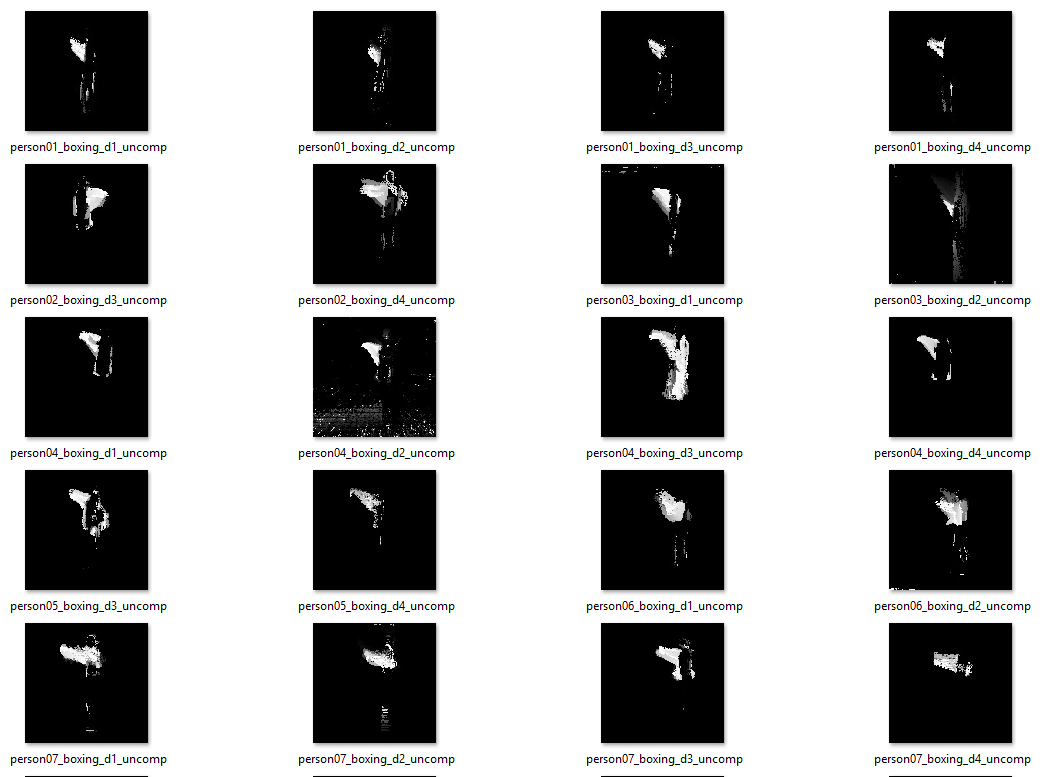
\includegraphics[width=15cm]{img/MHIbox.png}
  \caption{Predspracované videá boxu.}
  \label{MHIbox}
\end{figure}  

Na obrázku \ref{MHIbox} môžme vidieť príklad už predspracovaných MHI prostredníctvom nášho algoritmu. Takto sme si vytvorili všetkých 600 obrázkov z pohybov na ďalší výber príznakov, ktoré sme uložili podľa typu pohybu do jednotlivých priečinkov s ich názvami. 

\subsection{Výber príznakov}
Keďže už máme predspracovaný obraz vo forme MHI, môžme pokračovať v extrahovaní príznakov z týchto obrazov. Na tento účel sme zvolili deskriptor HOG popísaný v časti \ref{HOGlabel}. Týmto spôsobom vytvoríme vektor príznakov, ktorý budeme môcť následne spracovať prostredníctvom PCA a tak ho dať trénovať do klasifikátora pre každý jeden pohyb z trénovacej množiny. Príznaky z každého MHI obrázku by mali byť v tvare vektora konštantnej dĺžky. 

\subsubsection{Príznaky HOG} \label{HOGim}
\begin{lstlisting}[
  caption={Algoritmus HOG},
  label={HOGcreate},
  language=python
]
image = cv2.imread('image.jpg', 0)

def hogCreate(image):
    winSize = (64,64)
    blockSize = (16,16)
    blockStride = (8,8)
    cellSize = (8,8)
    nbins = 9
    winSigma = 4.
    gammaCorrection = 0
    nlevels = 64
    hog = cv2.HOGDescriptor(winSize, blockSize, blockStride, cellSize, nbins, winSigma,            gammaCorrection,nlevels)
    winStride = (8,8)
    padding = (8,8)
    locations = ((10,20),)
    hist = hog.compute(image,winStride,padding,locations)
    arrVectorFinal.append(np.concatenate(hist))
\end{lstlisting}

V tomto algoritme \ref{HOGcreate} vstupuje do funkcie \textit{hogCreate} parameter \textit{image} je vlastne obrázkom, ktorý je výstupom funkcie\textit{imread} z knižnice OpenCV. Pre dobré vybratie príznakov je potrebné nastaviť a vytvoriť \textit{HOGDescriptor}, ktorý obsahuje viacero parametrov:

\begin{itemize}
\item winSize
\item blockSize
\item blockStride
\item cellSize
\item nbins
\item gammaCorrection
\item nlevels 
\end{itemize}

\textbf{winSize} parameter určuje veľkosť okna na detekciu, musí byť zarovnaný podľa \textit{blockStride} a \textit{blockSize}.

\textbf{blockSize} je veľkosť bloku v pixeloch. Má byť zarovnaný na veľkosť bunky \textit{cellSize}.

\textbf{blockStride} musí byť násobkom veľkosti bunky, znamená veľkosť kroku, ktorým sa blok bude posúvať.

\textbf{cellSize} je veľkosť bunky.

\textbf{nbins} je počet rozdelení uhlov do ktorých jendotlivé gradienty zapadajú.

\textbf{gammaCorrection} hodnota určuje, či sa má ppoužiť predspracovanie gamma úpravy alebo nie.

\textbf{nlevels} určuje maximálny počet detekčných okien, predvolená hodnota je 64.

Po takomto nastavení deskriptora HOG môžme následne spracovať vstupný obraz a vytvoriť tak histogram hodnôt, ktoré už sú reprezentovateľné príznaky, ktoré vložíme do vektora príznakov \textit{arrVectorFinal}. Konečným výstupom je teda pole vektorov, ktoré obsahuje príznaky extrahované zo všetkých testovacích videí. Už tento vektor vieme následne použiť pre trénovanie klasifikátora, avšak pre zlepšenie výsledkov ešte tieto dáta upravíme. Vektor týchto príznakov sme zložili z troch MHI obrázkov z jedného videa, ktoré boli spracované vo štvrtej, šiestej a deviatej sekunde, čo dokáže presnejšie identifikovať pohyb jednotlivých aktérov.


\subsubsection{Prídavné príznaky} \label{pridavny}
Ďalšími príznakmi, ktoré sme sa rozhodli vybrať do vektora príznakov sú priemery hodnôt jednotlivých polí pixelov. Týmto algoritmom sme chceli znovu navýšiť úspešnosť, keďže pohyby v jednotlivých triedach sa vykonávajú v rôznych častiach snímaného obrazu. Týmito hodnotami vieme určiť v ktorých častiach obrazu MHI sa vykonával pohyb a v akej intenzite. Pre tento algoritmu sme potrebovali zvoliť vhodné parametre: 
\begin{itemize}
\item Šírka okna
\item Výška okna
\end{itemize}

\textbf{Šírka okna} nám udáva počet pixelov, ktoré budeme spracovávať v jednom rade pixelov v iterácii.
\textbf{Výška okna} je potrebná na definovanie počtu pixelov spracovávaných v stĺpci pixelov v iterácii.

Tieto dva parametre je potrebné určiť ako delitele šírky (160px) a delitele výšky (120px) MHI obrázkov. V našej implementácii sme využili šírku a výšku s hodnotou 10.

\begin{lstlisting}[
  caption={Prídavné príznaky},
  label={FeatAdd},
  language=python
  ]
  HEIGHT = 10 
  WIDTH = 10
  
  def processImg(image, boxes):
    count = 0
    rowBoxNum = 120 / HEIGHT
    colBoxNum = 160 / WIDTH
    sumOfBox = 0
    additionalVector = []
    value = 0
        
    data = np.asarray(image.getdata()).reshape(image.size)
    
    for i in range(0, rowBoxNum):
        for j in range(0, colBoxNum):
            for row in range(i*HEIGHT, i*HEIGHT + HEIGHT):
                for column in range(j*WIDTH, j*WIDTH + WIDTH):
                    sumOfBox = sumOfBox + data[column][row] 
                    count = count + 1
            value =  float(sumOfBox)/(WIDTH*HEIGHT)/255
            additionalVector.append(value)
            sumOfBox = 0
    return additionalVector
]

\end{lstlisting}

V algoritme \ref{FeatAdd} je vo funkcii \textit{processImg} na vstupe obrázok MHI (\textit{image} a počet okien pixelov s rozmermi 10 x 10 pixelov na jeden obrázok. Obraz sme si pre zjednodušenie vložili do \textit{NumPy} poľa a následne iterovali. Aby sme získali normalizovaný príznak \textit{(z rozmedzia <0,1>)}, potrebovali sme vydeliť hodnotu príznaku z jedného okna hodnotou \textit{255}, keďže každý pixel nadobúda hodnoty\textit{<0,255>} podľa svietivosti pixelu.

\begin{figure}[H]
  \centering
  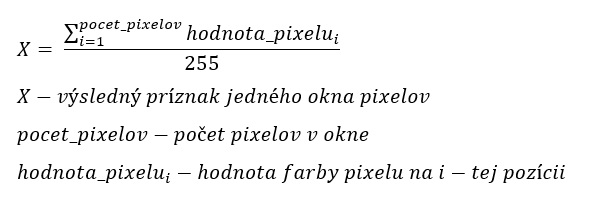
\includegraphics[width=10cm]{img/AddFeat.png}
  \caption{Výpočet príznaku okna pixelov}
  \label{MHIbox}
\end{figure}   

Takto vypočítané príznaky sme pridávali do vektoru príznakov na následné spracovanie a úpravu v PCA.

\subsubsection{Spracovanie pomocou PCA} \label{PCAim}
V algoritme \ref{PCAcreate} na extrakciu komponentov, ktorú sme si popísali v časti \ref{PCAlabel} sme použili metódy triedy \textit{\textbf{PCA}} knižnice \textit{sklearn}. Pre vytvorenie objektu PCA, sme použili parameter \textit{n\_components}, ktorý udáva počet komponentov, koľko chceme vybrať z vektora príznakov \textit{arrVectorFinal}. Tento počet komponentov musí byť nižší alebo nanajvýš rovný počtu vektorov príznakov. Natrénovaný model PCA s vektorom príznakov \textit{arrVectorFinal} sme uložili pre ďalšie spracovanie v SVM.

\begin{lstlisting}[
  caption={Trénovanie PCA},
  label={PCAcreate},
  language=python
]
pca = PCA(n_components)
pca.fit(arrVectorFinal)
joblib.dump(pca, 'ModelPCA.pkl')   
\end{lstlisting}

Trénovacia množina obsahuje 240 videí \textit{(6 tried po 40 videí)}, preto je aj maximálny počet hlavných komponentov, ktoré môžme získať z vektora príznakou pomocou PCA je 240. Teda výsledný vektor príznakov sa zmenšil na tie príznaky, ktoré sú najdôležitejšie. Neskôr v časti \ref{testalad} si ukážeme spôsoby, ktorými sme sa snažili naše výsledky ešte viac zlepšiť.  


\subsection{Klasifikácia}
Pre natrénovanie klasifikátora sme sa rozhodli použiť SVM, ktorý sme popísali v časti \ref{SVMlabel}. Na implementovanie SVM sme použili triedu \textit{svm} z knižnice \textit{sklearn}. K dátam, ktoré máme uložené v \textit{arrVectorFinal} potrebujeme ešte označenie, ktorý vektor do akej kategórie patrí. Preto sme vytvorili ďalší vektor, v ktorom je pre každé video označenie kategórie, kam vektor patrí. Teraz už môžme natrénovať SVM. 
\hfill \break
\begin{lstlisting}[
  caption={Trénovanie klasifikátora},
  label={SVMcreate},
  language=python
]
clf = svm.SVC(decision_function_shape='ovr')
clf.fit(arrVectorFinal, classVector)
joblib.dump(clf, 'Model.pkl') 
\end{lstlisting}
Algoritmus \ref{SVMcreate} využíva volanie funkcií \textit{svm.SVC}, ktoré nám vytvorí klasifikátor (angl. Support Vector Classifier), rozhodovaciu funkciu sme zvolili \textit{ovr} (angl. one versus rest), keďže máme viac ako dve triedy pohybov. Následne prostredníctvom funkcie \textit{fit} sme natrénovali klasifikátor \textit{clf}, kde boli vložené vektory príznakov \textit{arrVectorFinal} a vektor tried \textit{classVector}. Takto natrénovaný model bolo potrebné uložiť pre ďalšie použitie a testovanie. 

\subsection{Priebežné testovania a ladenie} \label{testalad}
Po naprogramovaní všetkých základných častí nášho projektu sme potrebovali otestovať naše riešenie, či náš klasifikátor funguje dobre a či môžme prejsť ku finalizácii výsledkov, prípadne k ďalším vylepšeniam a zmenám.


\subsubsection{t-SNE}
Aby sme vedeli výsledok trénovania našej SVM, potrebovali sme výsledky vizualizovať, ako prebehlo rozdelenie do tried. Na to sme využili testovací nástroj \textit{\acrfull{tsne}}, ktorého algoritmus nájdete v prílohe \ref{att:B}. Tento algoritmus umožňuje vizualizáciu viacrozmerných dát do 2D priestoru. Túto techniku je možné implementovať pomocou aproximácií, ktoré môžu byť aplikované na datasety obrovských rozmerov. Autorom tohto algoritmu je \textbf{\textit{Laurens van der Maaten}}, ktorý pôsobí ako výskumný pracovník na poli strojového učenia a počítačového videnia. t-SNE implementoval pre množstvo jazykov vrátane jazyka Python, takže sme nemali problém tento nástroj využívať. \cite{c18}



\subsubsection{Prvotné testy}
Ako prvý krok sme zvolili testovanie a tréning dvoch množín a teda beh a boxovanie. SVM sme natrénovali na tridsiatich videách z triedy behu a tridsiatich videách z triedy boxovania. 

Výsledok trénovania bol pre nás dobrý, keďže už vizuálne bolo vidno rozdelenie týchto pohybov do dvoch tried. Výsledok je možné vidieť na obrázku \ref{Test2Class}. 

\begin{figure}[H]
  \centering
  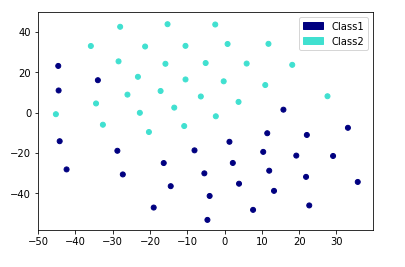
\includegraphics[width=14cm]{img/test2classes.png}
  \caption{Test dvoch tried pohybu}
  \label{Test2Class}
\end{figure} 


Ako príklad uvedieme taktiež pokus trénovania s jedným MHI, ktorý bol vytvorený vo 4. sekunde priebehu pohybu, avšak bez získania prídavných príznakov \ref{pridavny} a využitia metódy PCA.  Do tohto testu sme zapojili 5 tried pohybov, teda dataset KTH bez triedy pomalého behu, keďže sme usudzovali, že táto trieda sa dosť prelína medzi triedami behu a chôdze, čo sa ukáže aj na ďalších výsledkoch. 

Takto natrénované SVM sme znovu podrobili testu \textit{t-SNE}, kde výstup vyzeral ako na obrázku \ref{Test5Class1}, výsledky síce dávali zmysel, avšak rozdelenie jednotlivých tried nebolo až tak prehľadné ako sme si predstavovali. Triedy behu a chôdze pôsobia veľmi chaoticky, tak ako aj boxovanie s tlieskaním a zasahovaním kývania.

\begin{figure}[H]
  \centering
  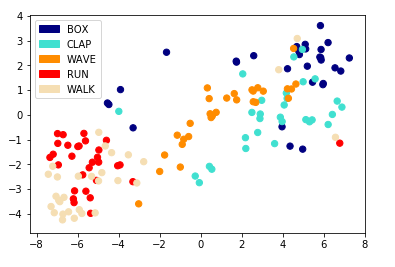
\includegraphics[width=14cm]{img/test5classes1.png}
  \caption{Prvý test piatich tried pohybu}
  \label{Test5Class1}
\end{figure}

Skúsili sme teda otestovať túto natrénovanú SVM, akú bude mať úspešnosť rozpoznávania. Výsledky môžte vidieť na obrázku \ref{Test5Class1g}.


\begin{figure}[H]
  \centering
  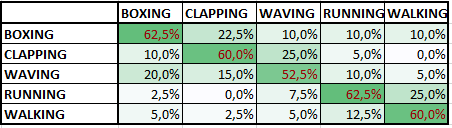
\includegraphics[width=14cm]{img/test5classes1tab.png}
  \caption{Úspešnosť 5 tried z 1 MHI}
  \label{Test5Class1g}
\end{figure}

Z tohto dôvodu sme sa rozhodli analyzovať náš postup a pristúpiť k optimalizácii riešenia, zbieraniu a ladeniu príznakov za pomoci viacnásobného využitia MHI, prídavných príznakov \ref{pridavny} a aplikovania PCA, ako bolo spomenuté v častiach \ref{HOGim}, \ref{PCAim}, \ref{pridavny}.


\subsubsection{Rozdelenie dát a finálne testy}
Dáta na tréning a testovanie sme rozdelili do dvoch skupín v pomere 40 testovacích videí a 40 trénovacích videí. Všetky testy boli vykonané na rovnakých videách, takže výsledky úspešnosti sú objektívne a porovnateľné pre každý typ konfigurácie programu.
Konfigurácie sme menili na 9 rôznych nastavení pre všetky triedy pohybov databázy KTH viď obrázok \ref{tabTesty}.

\begin{figure}[H]
  \centering
  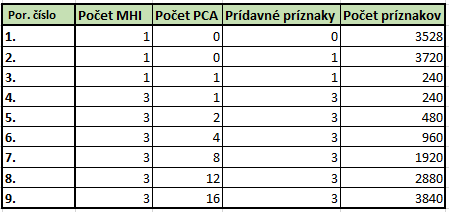
\includegraphics[width=14cm]{img/tabTesty.png}
  \caption{Testovacie konfigurácie}
  \label{tabTesty}
\end{figure} 

Ako vidno na obrázku, zvolili sme obmeny počtu MHI obrázkov s násobnými počtami vektorov pre získanie hlavných komponentov ako aj počet prídavných príznakov vypočítavaných z MHI. 

\paragraph{1. Test} 
V prvom teste s konfiguráciou jedného obrázku MHI, bez výpočtu PCA a prídavných príznakov sme dostali prvé výsledky \ref{test1}.

\begin{figure}[H]
  \centering
  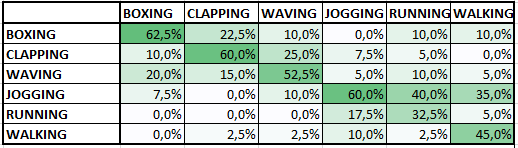
\includegraphics[width=14cm]{img/test6classes1g.png}
  \caption{Test č. 1}
  \label{test1}
\end{figure} 

Z výsledkov je viditeľný problém medzi triedou \textit{Running} a \textit{Jogging}, kde zo všetkých testovaných videí behu vyhodnotilo až 40\% ako pomalý beh a 35\% chôdze vyhodnotilo ako pomalý beh. 


\paragraph{2. Test} 
V druhom teste sme pridali ďalšie príznaky do vektora, výsledky pohybov sa zlepšili až na triedy behu, kde bol prepad až na úspešnosť 7,5\% a triedy behu, kde sa tiež znížila úspešnosť. Porovnanie je na obrázku \ref{test2}.


\begin{figure}[H]
  \centering
  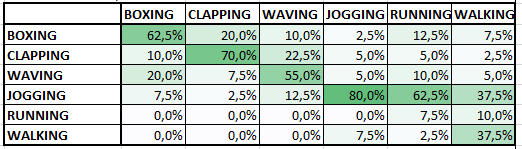
\includegraphics[width=14cm]{img/test6classes11g.png}
  \caption{Test č. 2}
  \label{test2}
\end{figure} 

\paragraph{3. Test} 
V tomto teste sme sa rozhodli zistiť vplyv PCA na celkové riešenie problému. Výsledky ukázali všeobecné zlepšenie, hlavne v triede mávania rukami, kde sa úspešnosť zvýšila z 55\% na 72.5\%.  
\begin{figure}[H]
  \centering
  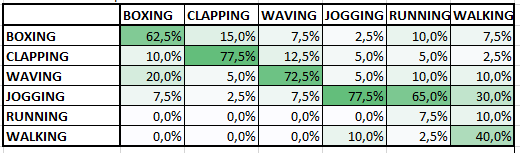
\includegraphics[width=14cm]{img/test6classes11PCA1g.png}
  \caption{Test č. 3}
  \label{test3}
\end{figure} 


\paragraph{4. Test} 
V nasledujúcich testoch nás zaujímal vplyv trojnásobného použitia obrázkov MHI na výsledky a úspešnosť testovania v spolupráci s rozširovaním PCA. Použili sme MHI z prvých 4, 6 a 9 sekúnd videa. Objavilo sa nepatrné zlepšenie až na prepad úspešnosti triedy \textit{Jogging}, v ktorom úspešnoť od predchádzajúceho testu klesla o 17,5\%. Finálny počet príznakov na jeden vektor bol 240.

\begin{figure}[H]
  \centering
  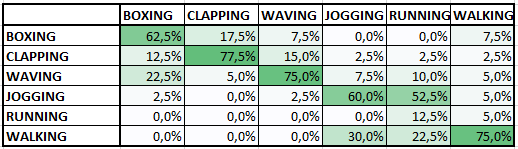
\includegraphics[width=14cm]{img/test6PCA1g.png}
  \caption{Test č. 4}
  \label{test4}
\end{figure} 

\paragraph{5. Test} 
V nasledujúcom teste sme iba zdvojnásobili počet vektorov príznakov videí (480 príznakov na video), aby sme mohli pomocou PCA vypočítať dvojnásobný počet príznakov ako v predchádzajúcom teste. Z výsledkov nám vyplynulo, že tento postup rozširovania počtu vektorov sa nám môže vyplatiť, keďže sa nám výsledky nezhoršili a v triede \textit{Waving} sme dokonca dostalo výsledok lepší o 2,5\%. 
\begin{figure}[H]
  \centering
  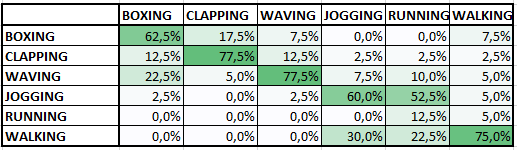
\includegraphics[width=14cm]{img/test6PCA2g.png}
  \caption{Test č. 5}
  \label{test5}
\end{figure} 

\paragraph{6. Test} 
Test so štvornásobne zvýšeným počtom vektorov (960 príznakov na video) nám znovu priniesol zlepšenie v triede \textit{Waving} a to dokonca o celých 5\%. Vzhľadom na to, že sa nám výsledky stále zlepšovali, snažili sme sa ísť ešte ďalej.
\begin{figure}[H]
  \centering
  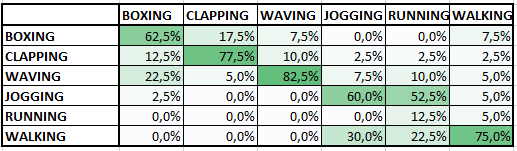
\includegraphics[width=14cm]{img/test6PCA4g.png}
  \caption{Test č. 6}
  \label{test6}
\end{figure} 

\paragraph{7. Test} 
Siedmy test s osemnásobným zväčšením počtu vektorov (1920 príznakov na video) nám znovu vylepšil výsledky o 2,5\% pre triedy \textit{Clapping} a \textit{Waving}. Stále to nemalo žiaden negatívny vplyv na ostatné výsledky.
\begin{figure}[H]
  \centering
  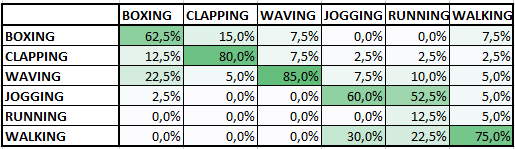
\includegraphics[width=14cm]{img/test6PCA8g.png}
  \caption{Test č. 7}
  \label{test7}
\end{figure} 

\paragraph{8. Test}
Pri teste, kde sme zvolili 12-násobné rozšírenie (2880 príznakov na video) počtu vektorov sa nám už zlepšovanie výsledkov zastavilo. Pri testoch sme namerali identické hodnoty, čo nám naznačovalo, že ďalšie zvyšovanie počtu vektorov nám už nebude naše výsledky vylepšovať.
\begin{figure}[H]
  \centering
  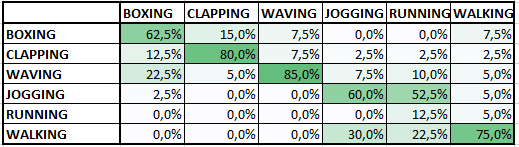
\includegraphics[width=14cm]{img/test6PCA12g.png}
  \caption{Test č. 8}
  \label{test8}
\end{figure}  

\paragraph{9. Test} 
Ako sme sa predpokladali, výsledky pri 16-násobnom rozšírení sa vôbec nezlepšili, naopak, v triede \textit{Jogging} sme zaznamenali pokles o 2,5\% z úspešnosti. 
\begin{figure}[H]
  \centering
  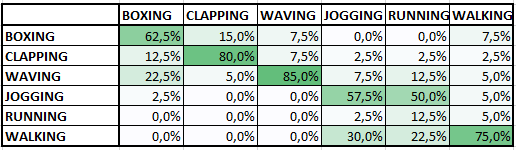
\includegraphics[width=14cm]{img/test6PCA16g.png}
  \caption{Test č. 9}
  \label{test9}
\end{figure} 

Pri tomto výsledku môžme povedať, že sme dosiahli maximum, ktoré sme mohli zvolenými metódami dosiahnuť. 

\section{Porovnanie s existujúcimi riešeniami}



